%======================================================================
\section{Escenarios extremos: ¿dónde está el riesgo? (F5a.3)}\label{sec:extremos}
%======================================================================
\paragraph{Por qué hacen falta.} En las familias nominal y estresada ningún controlador pasó
de 1185~K, ni siquiera sin ACS. Una capa de riesgo sobre un límite que nunca se acerca
estaría siempre inactiva y daría lo mismo que el MPC determinista. Antes de diseñarla hay que
saber en qué escenarios la seguridad está realmente en juego.

\paragraph{El límite que importa es 1220~K.} El monitor del DET clasifica la PCT en tres
estados: bajo 1180~K, en la banda [1180, 1220]~K y sobre 1220~K. En Simulink, el tercer
estado \emph{detiene la simulación}: es el estado final del árbol de eventos. Por eso las
corridas de esta sección terminan cuando la PCT cruza 1220~K, y ese cruce se cuenta como el
evento de falla. El límite $U_y=1244$~K de la función de costo queda más allá.

\paragraph{Barrido de severidad.} Primero se simuló sólo el HRM, con la lógica del DET, para
fugas cada vez más severas:

\begin{table}[H]\centering\small
\begin{tabularx}{\linewidth}{@{}Y r r r l@{}}\toprule
Fuga ($d$, $A$, $B$) & Activación & Fuga & PCT máx.\ (PI) & Sin ACS: 1180 $\to$ 1220~K\\\midrule
10, 0.28, 10 ($\approx$ archivada) & 1134~s & 4.7~kg/s & 1189~K & 1134 $\to$ 1649~s\\
15, 0.20, 10 & 823~s & 9.7~kg/s & 1198~K & 822 $\to$ 1065~s\\
20, 0.20, 15 & 724~s & 14.3~kg/s & 1206~K & 723 $\to$ 886~s\\
20, 0.10, 15 & 690~s & 17.2~kg/s & 1211~K & 688 $\to$ 823~s\\
30, 0.10, 10 & 629~s & 25.1~kg/s & --- & inventario agotado en 820~s\\\bottomrule
\end{tabularx}
\caption{Severidad de la fuga, sin MPC. ``Fuga'' es su magnitud en la activación del ACS y
``PI'' el controlador de respaldo del DET.}
\end{table}

\begin{itemize}
  \item Sin ACS, la PCT llega a 1220~K en 130--240~s con fugas severas, y en unos 500~s con
        la fuga archivada.
  \item El PI del DET contiene todas las fugas, con caudales de 370--530~kg/s, pero tarda:
        su integrador necesita unos 150~s para alcanzar el umbral de la bomba.
  \item Con fugas de 10--17~kg/s, la caja archivada (12.86~kg/s) ya no compensa la fuga.
\end{itemize}

\paragraph{La familia extrema.} Combina las dos fuentes de riesgo propuestas: (a)
escenarios más severos y (c) la caja archivada, cuya capacidad queda por debajo de la fuga.
Cada realización sortea:
\begin{itemize}
  \item fuga $d\sim U(15,25)$~kg/s, $A\sim U(0.1,0.2)$, $B\sim U(10,15)$;
  \item el inicio del MPC entre 0 y 17~s después de la activación (fase aguda);
  \item un ACS que entrega el 60--90\,\% de lo pedido y falla durante 30--90~s;
  \item un error del pronóstico de fuga de $-0.5$ a $0.1$~kg/s.
\end{itemize}
Se comparan, durante 240~s: sin ACS, caudal máximo constante, el PI del DET y N2 con y sin
sesgo con los dos actuadores. N1 y N3 se omiten porque coinciden con N2, y la referencia
pareada pasa a ser N2+sesgo.

\paragraph{Resultados} (14 realizaciones, \code{results/f5a2\_monte\_carlo/runs\_extreme.csv}).

\begin{table}[H]\centering\footnotesize\setlength{\tabcolsep}{4pt}
\begin{tabularx}{\linewidth}{@{}l Y r r r r@{}}\toprule
Actuador & Controlador & Llega a 1220~K & Tiempo hasta 1220~K & PCT máx.\ si no llega & Masa inyectada\\\midrule
--- & Sin ACS & 14/14 & 113--181~s (media 140) & --- & 0\\
Archivado & Caudal máximo, N2, N2+sesgo & 9/14 & 155--251~s (media 191) & 1206--1219~K & 470--2070~kg\\
--- & PI del DET & 0/14 & --- & 1204--1216~K & 5300--6360~kg\\
Físico & N2 / N2+sesgo & 0/14 & --- & 1189--1207~K & 3260--5170~kg\\\bottomrule
\end{tabularx}
\caption{Familia extrema. Los tiempos se cuentan desde la activación del ACS. Las tres
variantes con la caja archivada dan resultados idénticos en las 14 realizaciones. Tiempo p99
por consulta de N2: $\le0.19$~s, sin fallas del solver.}
\end{table}

\begin{figure}[H]\centering
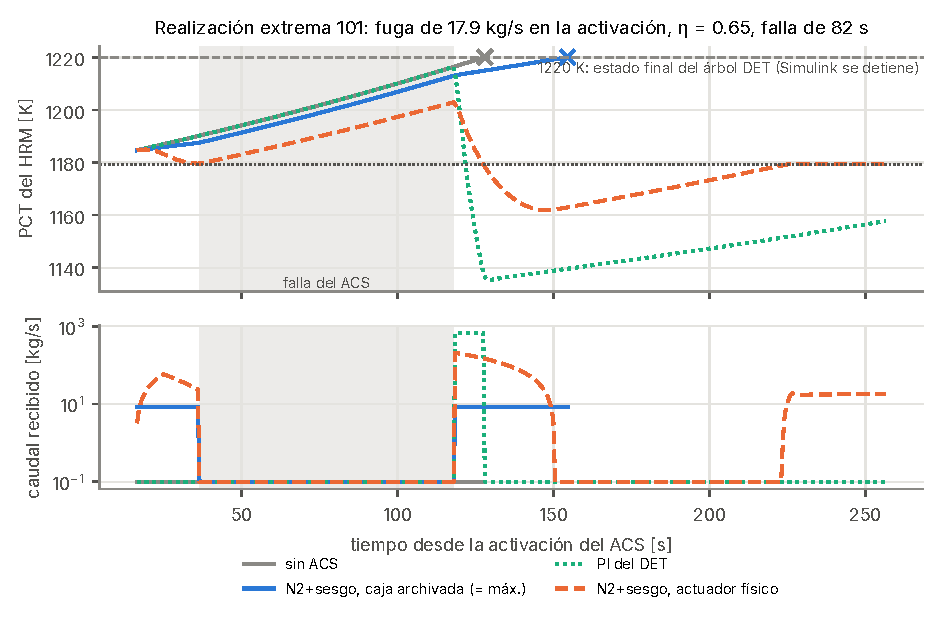
\includegraphics[width=\linewidth]{figures/fig_cl_extreme.pdf}
\caption{Una realización extrema. Sin ACS, la PCT llega a 1220~K a los 128~s (cruz gris). Con
la caja archivada, el MPC satura en todo momento (igual que el caudal máximo) y sólo retrasa
el cruce hasta los 155~s (cruz azul). El PI del DET reacciona tarde pero con fuerza (hasta
670~kg/s) y enfría hasta 1135~K. N2 con el actuador físico deja subir la PCT durante la falla
hasta 1203~K y vuelve a la referencia sin sobreenfriar.}
\end{figure}

\begin{figure}[H]\centering
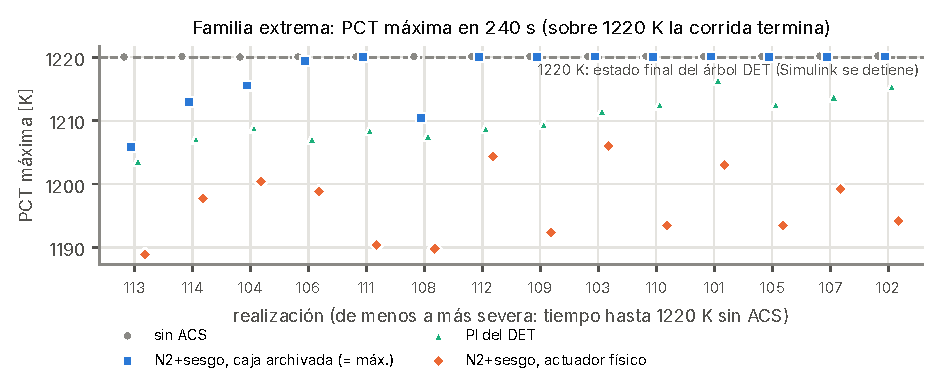
\includegraphics[width=\linewidth]{figures/fig_cl_extreme_max.pdf}
\caption{PCT máxima por realización. Los puntos sobre la línea de 1220~K son corridas que
alcanzaron el estado final del DET.}
\end{figure}

\paragraph{Cómo leer estos resultados.}
\begin{enumerate}
  \item \textbf{Con la caja archivada, el optimizador no importa.} En las 14 realizaciones
        el MPC decide el caudal máximo en cada consulta: la fuga supera la capacidad. N2, N2
        con sesgo y el caudal máximo constante dan exactamente la misma trayectoria, y 9 de
        14 llegan al estado final del DET, en promedio unos 60~s después de lo que llegarían sin ACS. Una
        capa de riesgo tampoco cambiaría nada: no hay decisión que tomar, sólo capacidad.
  \item \textbf{Con el actuador físico, el límite queda lejos.} Ninguna realización pasa de
        1207~K, aun con fallas de hasta 90~s y un ACS al 60\,\%. El margen mínimo es de 13~K.
        El MPC inyecta un 25\,\% menos de masa que el PI del DET y no sobreenfría.
  \item \textbf{La corrección de sesgo pierde precisión con fallas del ACS.} El calentamiento
        del ROM usa los caudales \emph{pedidos}, así que el gemelo no sabe que el ACS falló.
        La corrección de sesgo absorbe esa diferencia, pero como un sesgo constante: en esta
        familia, N2 con y sin sesgo no se distinguen ($\Delta$ISE $=-16\,000\pm21\,000$~K$^2$).
        Si el caudal real del ACS se mide, el gemelo debería usarlo.
\end{enumerate}

\takeaway{El riesgo de cruzar 1220~K existe en esta familia, pero en los dos actuadores
probados no depende de la decisión: con la caja archivada nada lo evita, y con el actuador
físico nunca ocurre. La capa de riesgo sólo puede aportar en el régimen intermedio, con una
capacidad comparable a la fuga y fallas largas del ACS. Ahí conviene mantener un margen bajo
la referencia ante una falla posible. Ése es el banco de pruebas que debe tener F5b.}

%======================================================================
\section{Lo que esto implica para la capa de riesgo}\label{sec:implicancias}
%======================================================================
\begin{enumerate}
  \item \textbf{Dónde montarla: sobre N2.} N1, N2 y N3 dan las mismas decisiones en lazo
        cerrado. N2 es un QP de $\sim30$~ms, así que admite escenarios y restricciones de
        riesgo sin salir del tiempo real.
  \item \textbf{Qué riesgo: cruzar 1220~K}, el estado final del DET, en escenarios con
        capacidad del actuador comparable a la fuga y fallas largas del ACS. El primer paso es
        un barrido de capacidad (15--50~kg/s con rampa dura) para ubicar ese régimen.
  \item \textbf{Corrección de la PCT: se mantiene $p_4$ con sesgo.} En la arquitectura de
        caja gris del gemelo, la parte de caja negra que corrige la PCT del ROM es el
        polinomio $p_4$, no la BiLSTM. Tras la corrección de sesgo, el desajuste ROM--HRM es
        $\le0.12$~K. Reentrenar una red sobre la diferencia de PCT entre el HRM y el modelo de
        caja blanca no se justifica con un residuo de ese tamaño.
  \item \textbf{Pronóstico de fuga: la BiLSTM, con su error modelado.} La réplica del HRM le
        entrega las mismas entradas que Simulink (fuga y $T_{e,c}$ del nodo 12), así que no hace
        falta ajustarla para usarla con la réplica. Sí haría falta en la familia extrema, que
        queda fuera de su rango de entrenamiento ($A\sim U(0.2,0.4)$, $d\sim U(8,10)$). El
        orden propuesto es: un modelo de error calibrado sobre sus residuos, un ajuste
        paramétrico de la ley de Park como alternativa sin red y, sólo si las decisiones de
        riesgo resultan sensibles al pronóstico, un ajuste fino con datos de la réplica.
  \item \textbf{Cómo evaluarla:} en forma pareada contra N2+sesgo, midiendo la frecuencia del
        cruce de 1220~K, la PCT máxima, el margen y el costo de la prudencia (masa inyectada y
        error de seguimiento).
\end{enumerate}

